%% ================================================================================
\chapter{Theory}
\label{ch:theory}
%% ================================================================================

%
%\begin{figure}
%  \centering
%  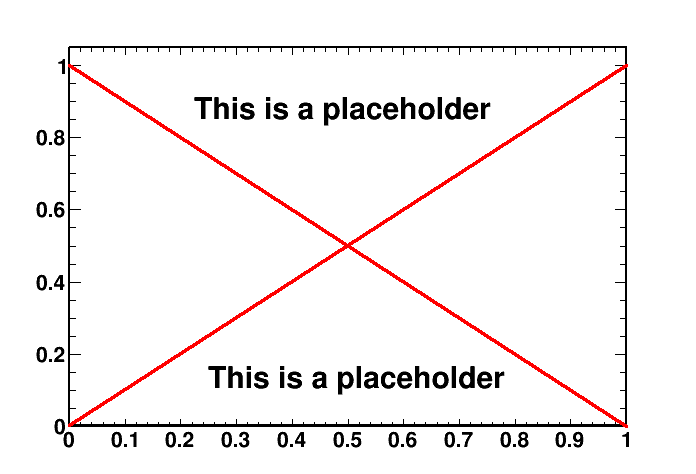
\includegraphics[width=.9\linewidth]{pic/dummy.png}
%  \caption{This is a dummy plot.}
%  \label{fig:dummy}
%\end{figure}
%
%\section{A section}
%\label{sec:section}
%Here we have Section \ref{sec:section}. \todo{This is a TODO marker} You might need this.

\section{Our Milky Way}

\subsection{General properties}


\begin{figure}[h]
  \centering
  \begin{minipage}[h]{0.45\textwidth}
  	\centering
	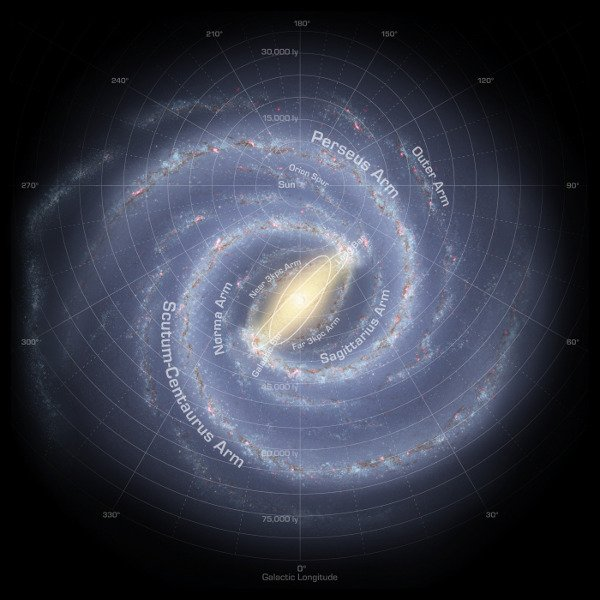
\includegraphics[width=1.\linewidth]{pic/theory/top_galaxy_map.jpg}
  	\subcaption{source: http://galaxymap.org/drupal/node/171}
  	\label{fig:top_gal_map}
  \end{minipage}
  \hfill
  \begin{minipage}[h]{0.45\textwidth}
	  \centering
	  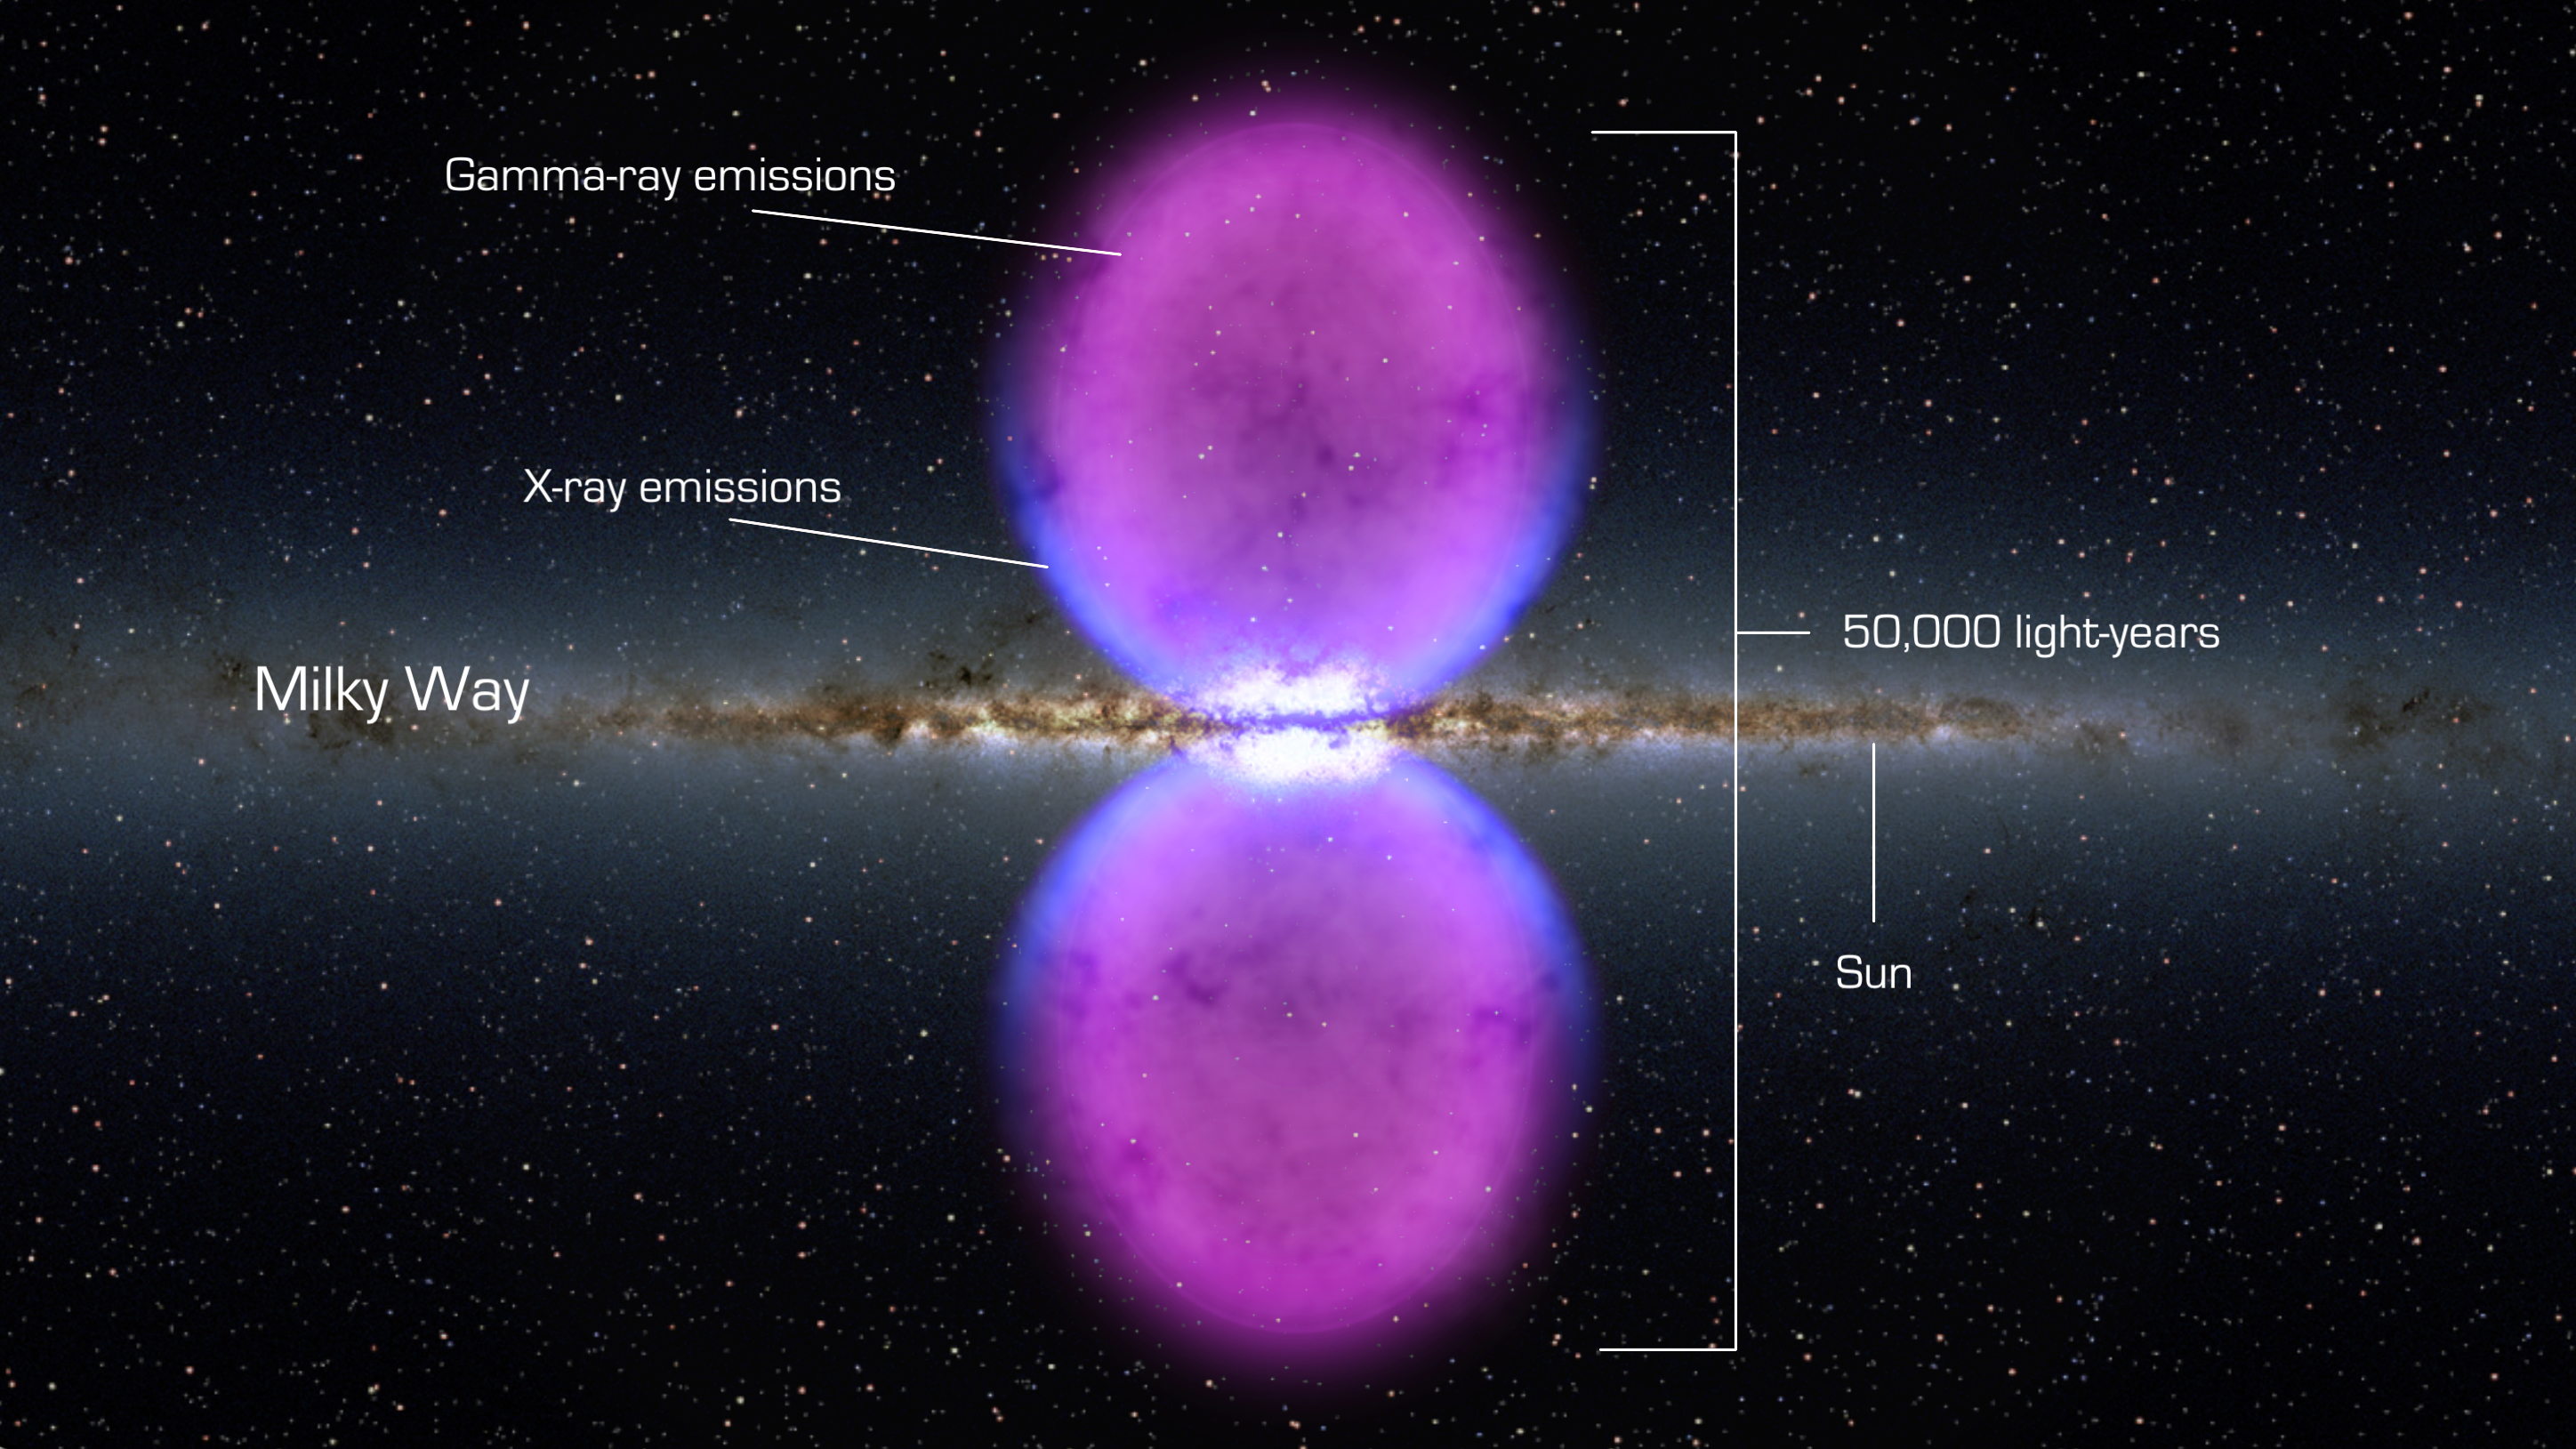
\includegraphics[width=1.\linewidth]{pic/theory/Fermi_bubble.jpg}
	  \subcaption{source: NASA's Goddard Space Flight Center}
	  \label{fig:fermi_bubbles}
  \end{minipage}
  \caption{The Milky Way, as seen from two different angles. (a) As seen from "above", the barred spiral arm structure is visible. As seen from Earth, the central bulge extend from circa -20 to 30 degrees. (b) Looking from the side, the disk is very thin, especially stars and dust, but gas is thicker, as well as the bulge. Two large bubble-like structures extends north and south from the galactic center, composed of high energetic particles.}
  \label{fig:Galaxy_maps} 
\end{figure}

For a long time, people thought the universe was constituted of only one galaxy, the Milky Way, the one in which the Sun and the Earth orbit. The discoveries of other galaxies in the universe came only in the 20's thanks to Edwin Hubble \cite{Hubble1925}. There are still unanswered questions about these objects, but the Milky way is well known and will play a major role in the focus of this thesis. Its shape, density and composition are three main factors playing a role in cosmic ray physics and cannot be avoided.

The Milky Way is a barred spiral arm galaxy, meaning it has two main spiral arms, connected in their center by a straight galactic bar. Those arms and bar are defined by a higher matter density, due to the orbits of stars around the center. Its diameter exceeds 40 kpc for a mass of around $10^{12} M_\odot$ and a thickness of under 1 kpc \cite{Kafle2014}. The Sun and the Earth are orbiting 8 kpc from its center, doing a complete rotation in 240 Myr.
All the different objects of the galaxy can be found in this thin disk of matter, mainly in the spiral arms. It includes the stars, planets and other massive objects, but also dust and gas clouds. As seen from Earth, the disk looks like a narrow band, a few degrees wide, but with a very high concentration of stars, gas and dust.
In 2010, two large scale structures were detected to the north and the south of the galactic center (GC) \cite{Slatyer2010} \cite{Ackermann2014}. With a diameter of 7 kpc, these two "bubbles" extend up to 40 degrees in latitude and 20 in longitude. They are a source of high energy gamma-rays and were detected by the Fermi Large Area Telescope (LAT) (Fig. \ref{fig:fermi_bubbles}).

The disk of the Milky Way is composed of matter in different forms, like stars, gas or dust. Stars are one of the main source of the interstellar radiation field (ISRF). They can be modeled as black body radiating at different energies depending on their temperature. They are the main source of ultra-violet (UV) photons that play a major role in gas evolution and composition. Stars are forming inside gas and dust clouds collapsing on themselves under their own gravitational pressure.
The gas is mainly composed of hydrogen, but heavier elements and even molecules can be found at the center of large dust and gas clouds where UV light cannot penetrate. One of these is the CO molecule, often used as a tracer of molecular clouds \cite{Planck2014} \cite{Liu2013}. Molecular clouds (MC) will be used to designate large regions of gas and dust which can possibly contain stars inside.
\todo{add gas/dust ratio} Dust is also present in the galactic disk. It can be warmed up by starlight, and then radiates infrared (IR) light. This IR source also contributes to the ISRF.

An electromagnetic field is present all across the milky way, generated by rotating stars, molecular clouds, or plasmas. It has been observed and measured, but it is complex and has no distinct direction at small scales (interstellar scale). Its complexity makes it impossible to measure precisely in every point of the galaxy, and impossible to model. The most common representation at small scales is still given by a random field direction.

\subsection{Dark Matter}

\begin{figure}[h]
 \centering
 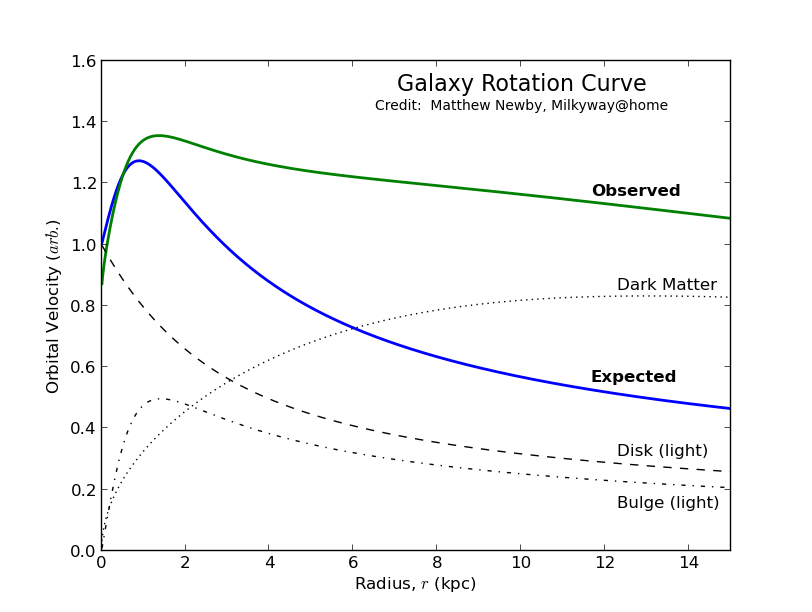
\includegraphics[width=.5\linewidth]{pic/theory/gal_rotation_curve.png}
 \caption{Orbital velocity of the Milky Way as a function of the distance from the GC. A clear discrepancy between the expected (in blue) and the observed (in green) velocity can be seen above a 2 kpc radius. The expected velocity drop too low above 2 kpc, when the observations show a flat curve. The blue curve is the sum of the predictions from the disk and the bulge, both composed of standard matter. But adding the predictions for dark matter to the blue curve, the theory would match much better the observations. \cite{Newby2018} \cite{Rubin1971}}
 \label{fig:gal_rotation_curve}
\end{figure}

The shape of spiral galaxies is well known today, with thousands of observed examples throughout the universe. This knowledge is used to mathematically model them, and in particular the rotation speed as a function of the distance respective to the center. It was a big surprise when the observed angular speed did not match the theory \cite{Rubin1971}, as shown in figure \ref{fig:gal_rotation_curve}. The expected curve (in blue) shows a decreasing rotation speed above a 2 kpc radius, while the observed curve (in red) flattens out and falls off steeply.
One of the explanation for this difference is the introduction of dark matter (DM), which brings a lot of invisible mass into the galaxy. It still is not observed and a few theories exist on its exact nature \cite{Hira2017}. Even if its exact nature is not known, its mass distribution can be deduced from the observed rotation curve of the galaxy. The predicted distribution is a spherical halo extending beyond the 40 kpc of the galactic disk. Its density peaks in the GC, and decreases with the radius following a given density profile. The exact profile is not known. A currently investigate parametrization of it is the Navarro-Frenk-White (NFW) profile defined as follows :

\begin{equation}
\rho (r) \propto \frac{1}{\left( r/r_S \right) \left( 1 + r/r_S \right)^2 }
\end{equation}

where $r_S$ is the scale radius, determining the size of the halo. \cite{NFW1997}


One of the most popular explanations of DM is the Weakly Interacting Massive Particles (WIMP) theory \cite{Jungman1996}. These particles are supposed to be non-standard particles with a large mass, neutral, and only sensitive to the weak force, making them difficult to observe. No particles of the standard model are valid candidates, or could provide the amount of mass needed to speed up a galaxy.
It is predicted that two WIMP colliding could produce gamma-rays, providing enough mass and energy. This gamma ray radiation is proportional to the WIMP density and cross-section, thus following the DM halo distribution.

\newpage
\section{Spectrum description and vocabulary}
%Energy spectra
%Intensity, Flux

To speak about CRs, one often speaks about their spectral shape, or energy spectrum. These terms refer to the energy flux $\Phi$ in GeV\textsuperscript{-1}.s\textsuperscript{-1}.cm\textsuperscript{-2}.sr\textsuperscript{-1} as a function of their energy. It describes how many particles of a given energy would be observed in a second by a one centimeter square instrument. This can often be modeled by a power law of the form $\Phi \propto E^{-\alpha}$  where $\alpha$ is called the spectral index. Lower values of $\alpha$ results in a "hard" spectrum, because of the important proportion of high energetic particles. This designation comes from the fact that the path of highly energetic particles are "hard" to bend. On the contrary, a "soft" spectrum has a bigger spectral index and describe a lower density of high energy particles compared to low energies. The terms "soft" and "hard" can be applied to any kind of energy spectrum, even if it is not a power law, it will only describe the relative proportion of high and low energy particles.

In the following chapters though, the preferred representation of the energy distribution is via the energy flux, or spectral energy distribution in GeV.s\textsuperscript{-1}.cm\textsuperscript{-2}.sr\textsuperscript{-1}, simply obtained by multiplying the particle flux by its energy square ($E^2 \times \Phi(E)$). In other terms, how much energy does the instrument receive every second for particles of a given energy. This is only done to facilitate the reading of the graphs and does not affect the underlying physics.



\newpage
\section{Physics of Cosmic Rays}

\subsection{Creation of CR}
\label{sec:creation_of_CRs}
%		-supernovae (SNR)
%		-AGN (activ galactic nuclei)
%		-pulsars, quasars

Several sources of Cosmic Rays exist in the universe. CR can be highly energetic and thus can only be produced by large astrophysical bodies. Particularly powerful events are supernovae, ejecting relativistic particles during the burst. The dying star ejects a lot of its mass, forming a supernova remnant (SNR) surrounding either a white dwarf, a neutron star or a black hole depending on the initial mass of the star. These SNR could also play a role after the explosion via the Fermi process; it is to say that an already energetic particle would bounce in the shock wave created by the explosion, and gain energy via magneto-hydrodynamic processes before escaping when a threshold energy is attained. \cite{Wu1984}
Another important source of CR are pulsars. These rapidly rotating neutron stars and their intense electromagnetic field accelerate high energy particles such as protons and electrons. This can last as long as the pulsar rotates fast enough, from 10 to 100 Myrs, before slowing down.
A third source are the actives galactic nuclei (AGN), also known as quasars. These objects consist of a super-massive black hole at the center of a galaxy. First discovered thanks to their radio emission, they are also able to eject CR, via Fermi or centrifugal acceleration.


\subsection{Propagation of CR}
%Propagation through the galaxy
%	-random B field -> no way to backtrace a CR
%	-interaction, shocks in MC
%	-Diffusion coefficient
%		-Can be different in disk, bubbles, or outside
%	-different diffuse coef mean different densities
%		-in MC, bubbles, outside
%		-can observe this inhomogeiniies via gamma rays

Once they are emitted, the CR propagate through the galaxy under the influence of different interactions.
The first thing to consider is the complex magnetic field running through the galaxy, originating from stars and molecular clouds or any distribution of charged particles. It is not particularly strong, on the order of micro-gauss \cite{Daniel1975} \cite{Farrar2012}, compared to the heliosphere or what can be created on Earth \cite{Gleeson1968}, but its very large scale suffice to bend the CR's path in all direction until the point where it is impossible to backtrack their origin.
Another possible interaction is the collisions with other particles. It depend on the density distribution of those colliders along the path of CRs. For example, a higher number of collisions in the disk is expected, where the density of molecular clouds is the highest.


\todo{give diffusion formula} All these influences can be modeled by a diffusion model, mainly defined by its diffusion coefficient D, which describes the average distance away from the origin traveled by the particles during a certain time. The higher the coefficient, the faster a particle will diffuse in the galaxy. On the contrary, if D is small, the particle's path will be bent in every direction so often that it stays close to its source for a longer time. 
%Each phenomenon can be attributed one of those coefficient to describe its effect on the cosmic rays, and adding them up gives the effective coefficient. \todo{give values for Dmag, Dcoll...}
While the diffusion coefficient for the galactic magnetic field can be taken as constant throughout the Milky Way \cite{Farrar2012}, the diffusion coefficient due to collision is proportional to the particles density. A smaller coefficient in molecular clouds is expected, where the density can reach \todo{value!}. \cite{Crutcher2012}

This coefficient will also define the CR densities in various locations of the galaxy. Indeed, the more a particle's path is twisted and convoluted, the longer it will take to move away from its origin. This way, a higher density of CR can be found in low diffusion coefficient areas like molecular clouds. In comparison, the region outside the galactic disk has a low density of CR due to a weak electromagnetic field and small gas and dust density.
However, the bubble region is outside the disk and has a higher concentration of high energy CR than other regions outside the disk. This is due to a direct outward emission of CRs from the GC region. With a high diffusion coefficient, these CRs are ejected light years away (see Fig. \ref{fig:fermi_bubbles}), forming two symmetric regions extending north and south up to 40 degrees in latitude in galactic coordinates.\cite{Ackermann2014}

The consequences of such diffusion processes is an isotropic CR sky on Earth. In whatever direction the instruments look at, they measure the same CR flux. This complicate CR study, since no information about their origin or their journey can be learned from direct observation, and it is why gamma-rays are useful in indirect detection methods.

\subsection{Energy losses}

Traveling through the galaxy particles interact with different objects and can gain or lose energy during the event. Every time a particle collides with another less energetic particle, or is deflected by a magnetic field, it loses energy. Depending on its energy and its surroundings, a particle will not always lose energy at the same rate.
If the particle has a high enough energy, it will mainly encounter lower energy particles and will lose energy faster than low energy particles. If a particle is in a molecular cloud, where all other particles have the same energy, every collision will only change its energy a little, and it will basically stay the same.
This process is important to explain changes in CR spectral index. The high energy particles emitted directly at the source will lose energy faster than the less energetic ones, populating the lower part of a spectrum. This way, a propagated population of CR has a softer spectrum than it had when emitted by its source. The theoretical index values for a propagated spectrum is 3.85, with a value of 2.1 for a source spectrum. \cite{Hillas2005}
This softening occurs more quickly in the disk, where a lot of collision happen, and more slowly perpendicular to it.

\todo{add picture of energy losses (see alexander thesis)}


\subsection{Effect of molecular cloud}

Molecular clouds could play a major role in the spectral distribution of CR in the disk via their magnetic field. 
A stronger magnetic field around those objects deflect the charged particles. If the CR particle has a high enough rigidity, the effect will be negligible, but for lower rigidity, the particle's path can be bend enough so that the particle never enters the MC.

Another theory is investigated. The electromagnetic field density in their core is greater than on the outside due to a higher density of particles. A particle entering the MC along a field line could be reflected by this increasing field density, much like it is observed on Earth with the Earth magnetic field.

\todo{cite on earth, in MCs}
\todo{add picture of the phenomenon}

In both cases, the result is the same. Low energy CR are deflected before entering the MC, thus hardening the lower energy CR spectrum in MCs.





\subsection{CRs as observed from Earth}

\begin{figure}[h]
 \centering
 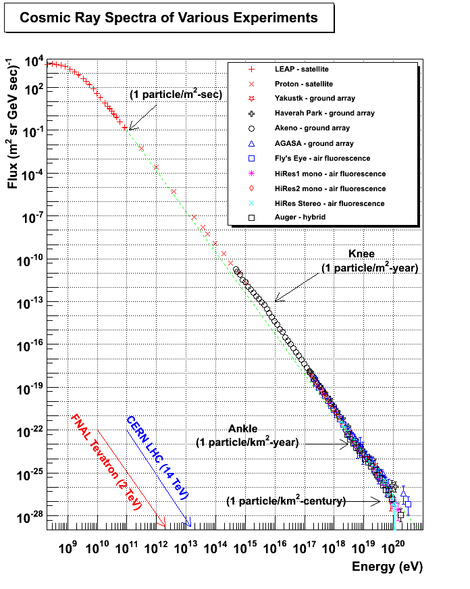
\includegraphics[width=.5\linewidth]{pic/theory/CR_spectrum.png}
 \caption{Cosmic ray spectrum as seen by several experiments. This characteristic shape can remind a leg, with a "knee" around $5.10^{15} eV$ and two different spectral indexes on both sides. Below $1^{10}$ eV, the spectrum flattens due to the solar and earth magnetic field which deflect lo energy particles. On the other side of the spectrum, above $1^{18}$ eV, the spectrum hardens imperceptibly, and the statistics are very low, but it is the highest energetic particles ever observed. In comparison, the red and blue arrows show two of the best human attempts to recreate very high energetic particles and give an idea how powerful CR can be. Source: http://www.physics.utah.edu/~whanlon/spectrum.html}
 \label{fig:CR_spectrum}
\end{figure}

The CR spectrum obtained from observations on Earth is shown in Figure \ref{fig:CR_spectrum}. It is the same in every direction as far as the measurement uncertainties can tell \cite{Hillas1984}. The isotropic arrival direction of CRs is measured with great care and any anisotropy, if existing, is below the instrument precision.
The CR spectrum is composed of three main features that form a "leg". The "knee" around $10^{7} GeV$ marks the separation between two different power laws in $E^{-\alpha}$. A slightly harder one below that is thought to be composed of galactic CRs, and a softer one above that is supposed to be of extra-galactic origin. The spectral index changes from 2.7 below to 3 above, due to different production mechanisms. \cite{Biermann1995}
As indicated on Figure \ref{fig:CR_spectrum}, the corresponding flux of particles is lower and statistical fluctuations are not negligible at high energies. Especially at the "ankle", above $10^9 GeV$, where only very few particles are detected.


\section{Physics of gamma-ray}

\subsection{Gamma-ray creation}
%		-pion decay
%		-bremmstrahlung
%		-inverse compton

Since the cosmic rays observed on Earth are hard to backtrack, some indirect detection methods are required to find their origin.CRs interact in a lot of ways with their environment, as described in the previous section. These interactions can leave detectable traces. The most common is the production of gamma-rays, i.e. photons in the GeV energy range. Once created, these gamma rays can be blocked or absorbed, but not deflected, which make them easier to backtrack. Linking gamma-ray and CRs requires to know the main production processes.

\subsubsection{Pion decay (PCR)}
%Explain phenomenon
%Explain expected gamma ray spectrum, propagated proton distribution.

%The high energy protons can produce $\pi^{0}$ which decay almost immediately in 2 gammas of equal energy.

Hadronic CRs  particles interact with the interstellar medium and can lead to $\pi^0$ production. Any CR nuclei can result in pion production, but since protons are the most abundant particles, they will dominate the production. 
These newly created pion can rapidly decay into a pair of gamma-rays (99\% of the time) or e\textsuperscript{+}e\textsuperscript{-} pairs, the latter being negligible.




\subsubsection{Bremsstrahlung (BR)}
%Explain phenomenon
%Explain expected gamma ray spectrum


A charged CR passing near another charged particle of the ISM or in a magnetic field will be deflected by the electromagnetic interaction. In the process, the CR will lose energy via the emission of photons. The emitted energy depends on the energy of the electron and the intensity of the electromagnetic field. The more the electron is deflected, the higher the energy of the emitted photons.
Even though proton CR are charged, the main sources of bremsstrahlung gamma-rays are electrons and positrons. This is due to the much lower mass of the electrons, making them easier to deflect. \todo{formula maybe}

\todo{give numbers for B field and proton in MC}


\subsubsection{Inverse Compton scattering (IC)}
%Explain phenomenon
%Explain expected gamma ray spectrum


%A third process can take create gamma-rays when the CR electrons interact with a photon of the interstellar radiation field (ISRF). 
When a high energy electron collides with a low energy photon, the electron transfers some of its kinetic energy to the photon, giving it enough energy to enter the GeV energy range.

The amount of gamma rays coming from Inverse Compton scattering is directly linked to the electron distribution and the ISRF of the galaxy. The latter is composed of three major components, the starlight, the dust emission and the cosmological microwave background (CMB). The first component is directly linked to the star distribution, and will be dominant in the disk, where most stars are located. The starlight follows a black body spectrum, peaking in the UV range. The dust emission comes from the infra-red emission of warm dust. It also is mainly present in the disk, following the matter distribution in the galaxy. Finally, the CMB is peaking in the microwave range but is uniformly present everywhere in the universe, and therefore in the galaxy. It is dominant where $\pi^{0}$ and BR are negligible, namely outside the galactic disk.


\todo{talk about synchrotron and ionization losses}

\subsubsection{Other sources}
%Gamma-ray burst
%Pulsars

The three previously described processes are general processes that can happen everywhere at any energy. Even though the processes are always the same, two classes of sources can be defined: the diffuse and the point sources.
The first correspond to all the CR propagating through the ISM and interacting with its components. It will be the object of study of the following chapters. 
The second are the gamma-rays produced directly at the CR origin (in SNR, AGN or pulsars as described in section \ref{sec:creation_of_CRs}). Every one of these sources should be studied separately and are not fully understood. Since these sources cannot be resolved by the instruments, they will be referred to as point sources in the following chapters. The spectral shape of these point sources is generally known and categorized as a function of the source type. This makes their recognition possible, and diffuse and point sources emissions can be separated.


%Other sources of gamma-rays exist in the universe that will complicate the observations. Gamma-rays are very energetic and thus can only be produced by very energetic phenomena. The gamma-ray bursts for example were discovered in the late 60's when U.S. satellites were build to detect nuclear weapon tests. These two events produce gamma-rays, but the first one is much more powerful, sometimes emitting more energy than the Sun will in its entire life-time. It is thought to be emitted by supernovae in distant galaxies or the merging of two neutron stars. These events are short (from milliseconds to hours) and will not be dominating the observations.
%An other source is the pulsar gamma-ray emission, and even though they are less energetic, their long-term production make them one of the first sources of observed gamma-rays. It can be said the same about quasars or active galactic nuclei (AGN).
%All these sources produce high energetic cosmic-rays that will lose energy via the different processes described earlier, and produce gamma-rays. 


\subsection{Gamma-ray observations}

On Earth, gamma-rays are absorbed by the atmosphere \cite{HSU}. To measure them directly, the instrument has to be launched into orbit above the atmosphere, where gamma-rays are not yet absorbed. The Fermi Large Area Telescope (LAT) for example, maps the gamma-ray sky between 20 MeV and 300 GeV \cite{Fermi2009}, detecting all the point source emissions as well as the diffuse background emission.


%The diffuse cosmic ray emission that we are interested in can be obtained after modeling and subtracting the contribution of the over sources. This allows us to compare the observation with the models we obtain from the previous three interactions.


In theory, the knowledge of the processes that generate gamma-rays from cosmic-rays and the precise composition of the Milky Way should allow to explain the observations. Propagation models and simulations are able to output the expected energy spectrum of gamma-rays reaching Earth from an initial distribution of cosmic-rays (not taking the point sources into account). When comparing the model and the observations differences arise, as will be discussed in the following section.


\newpage
\section{Unresolved problems of gamma-ray observations}
%What are the unresolved problems of the precedent sections:
%	-Bad fits in bubbles and disk	
%	-Spherical gamma-ray excess in GC when fitting spatial templates
%		-DM studies
%			-Hooper
%			-others...
%		-MSP studies
%			-Fermi
%			-Hooper
%			-Weniger
%	-High energy tail flux too hard
%	
%


%\begin{figure}
% \centering
% 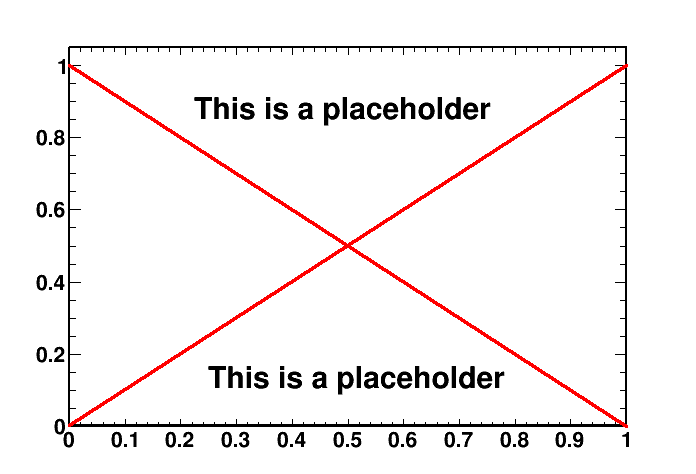
\includegraphics[width=.9\linewidth]{pic/dummy.png}
% \caption{chi2 distribution of first fits (not mines)}
% \label{fig:first_BKGonly_fits}
%\end{figure}
%
%
%
%\begin{figure}
% \centering
% 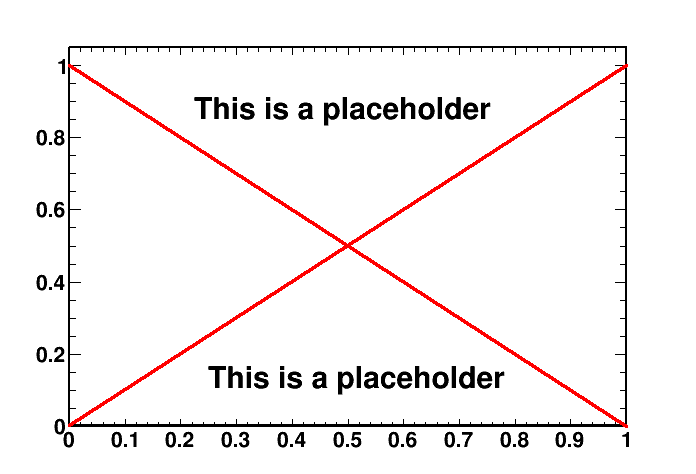
\includegraphics[width=.9\linewidth]{pic/dummy.png}
% \caption{shape of the excess}
% \label{fig:first_BKGonly_fits}
%\end{figure}

Several studies have already tried to see how the predictions of the gamma rays emission and the observations compare \cite{Calore2015}, \cite{Fermi2017}, \cite{Yang2016}. The three discussed processes were modeled to try to recreate the spectrum observed here on Earth. The accepted model is composed of a single spectrum of propagated proton CR, and a single electron spectrum. Then, gamma-rays are deduced and modeled from there. The results show discrepancies.
Even though the observations of the galactic poles or any high latitude regions can be well explained by a propagated CR, bremsstrahlung and inverse compton scattering component, the models fail to reproduce the surroundings of the galactic disk, and in particular the GC or the bubbles. 
Two discrepancies can be identified. A high energy deficit in the models, where the observed high energy tail (> 50 GeV) cannot be reproduced \cite{Yang2016}, and a spherical excess centered in the GC around 2 GeV.

The first one shows a lack of high energy CRs in the models. A mean of injecting more relativistic particles has to be found in order to fill this gap. One explanation is that we do not observe only diffuse emission in the disk. The point source emission could not be entirely subtracted due to the high density of sources. The CRs that did not yet propagate have a harder spectrum, thus providing a higher ratio of high energy gamma-rays. This would also happen in the bubbles, were CR are injected without propagating in the disk first.

Two main ideas have emerged to explain the spherical excess.
First is the presence of dark matter in the galaxy in the form of weakly interacting massive particles (WIMP). The spatial distribution of these particles would follow a NFW profile centred at the GC. They are also expected to produce gamma rays when annihilating with each other via hadron production. In theory, if the mass of a WIMP particle is around 50 GeV, the expected gamma spectrum would peak around 2 GeV, where the excess is observed. \cite{Calore2015}, \cite{Fermi2017}
The study of the excess could put strong limits on the mass and annihilation cross section of such WIMPs and confirm, or reject the theory.
The second theory does not involve new physics, but unobserved millisecond pulsars. They would also be spherically distributed around the GC and their gamma spectrum peaks around 2 GeV. A few thousand of them would be needed to recreate the intensity of the excess \cite{Fermi2017}. The main default of this explanation resides in the fact that we have observed only a few hundreds pulsars so far when we expect ten times more to explain the excess.















